\subsubsection{Verbindungen zu Endsysteme einstellen}
\begin{figure}[!htb]
    \paragraph{VLAN 10 Verbindungen}
    \centering
    \begin{subfigure}{\textwidth}
        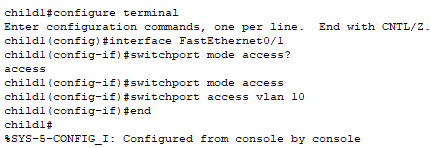
\includegraphics[width=\textwidth]{./img/Access1/users.png}
        \caption{Access1/child1}
    \end{subfigure}
    \begin{subfigure}{\textwidth}
        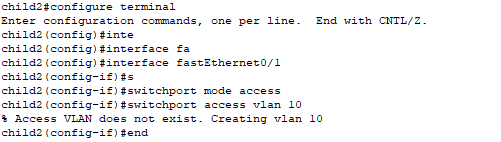
\includegraphics[width=\textwidth]{./img/Access2/users.png}
        \caption{Access2/child2}
    \end{subfigure}
\end{figure}

\begin{figure}[!htb]
    \paragraph{VLAN 20 Verbindungen}
    \centering
    \begin{subfigure}{\textwidth}
        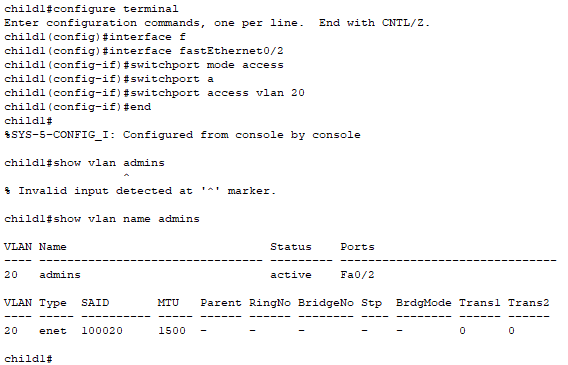
\includegraphics[width=\textwidth]{./img/Access1/admins.png}
        \caption{Access1/child1}
    \end{subfigure}
    \begin{subfigure}{\textwidth}
        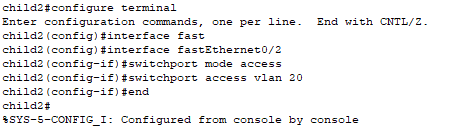
\includegraphics[width=\textwidth]{./img/Access2/admin.png}
        \caption{Access2/child2}
    \end{subfigure}
\end{figure}
\FloatBarrier

\clearpage
\pagebreak
\subsubsection{Ports einstellen}

\begin{figure}[!htb]
    \paragraph{Access1}
    \centering
    \begin{subfigure}{\textwidth}
        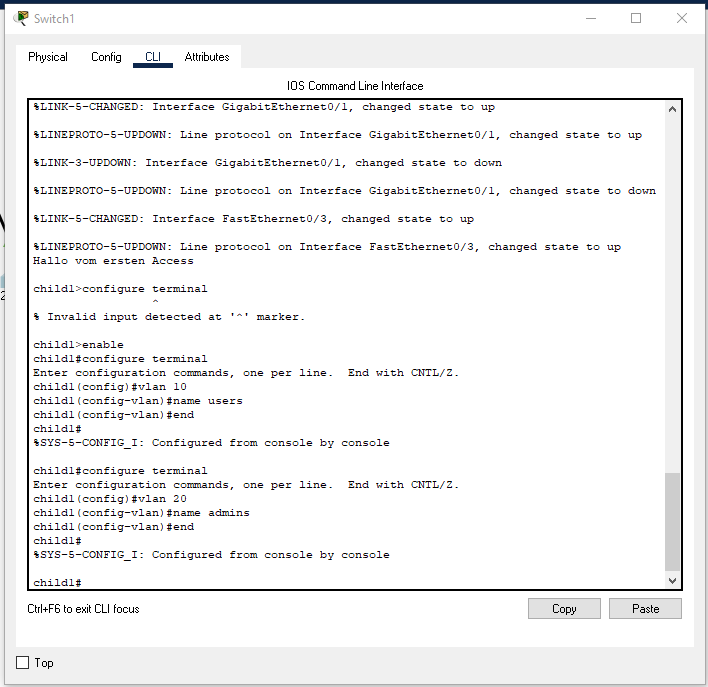
\includegraphics[width=\textwidth]{./img/Access1/vlan_10-20.png}
        \caption{Vlans registrieren}
    \end{subfigure}
\end{figure}
\begin{figure}[!htb]\ContinuedFloat
    \centering
    \begin{subfigure}{\textwidth}
        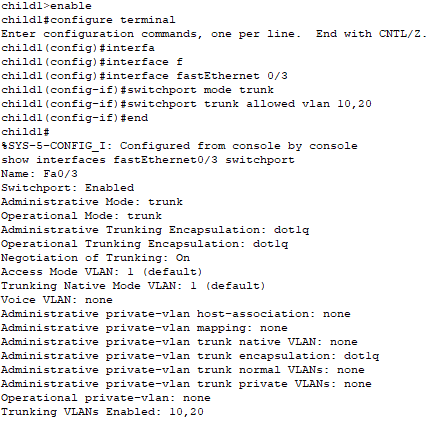
\includegraphics[width=0.95\textwidth]{./img/Access1/trunk.png}
        \caption{Trunk Port einstellen}
    \end{subfigure}
\end{figure}

\begin{figure}[!htb]
    \paragraph{Access2}
    \centering
    \begin{subfigure}{\textwidth}
        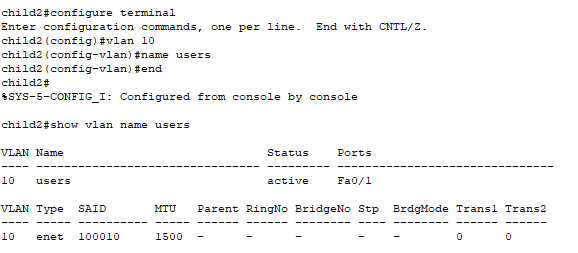
\includegraphics[width=\textwidth]{./img/Access2/vlan10.png}
        \caption{Vlan 10 registrieren}
    \end{subfigure}
    ~
    \begin{subfigure}{\textwidth}
        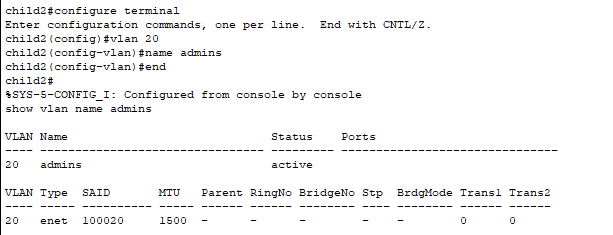
\includegraphics[width=\textwidth]{./img/Access2/vlan20.png}
        \caption{Vlan 20 registrieren}
    \end{subfigure}
\end{figure}
\begin{figure}[!htb]\ContinuedFloat
    \begin{subfigure}{\textwidth}
        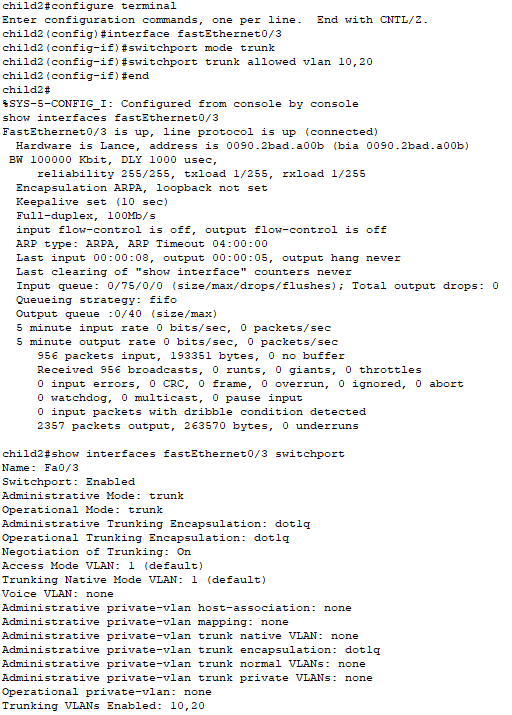
\includegraphics[width=\textwidth,height=.95\textheight]{./img/Access2/trunk.png}
        \caption{Trunk Port einstellen}
    \end{subfigure}
\end{figure}


\begin{figure}[!htb]
    \paragraph{Backbone}
    \centering
    \begin{subfigure}{\textwidth}
        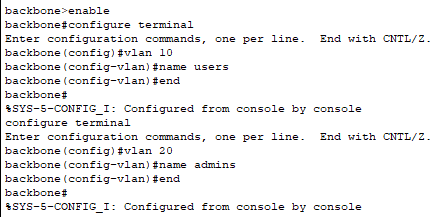
\includegraphics[width=\textwidth]{./img/Backbone/vlan.png}
        \caption{Vlans registrieren}
    \end{subfigure}
\end{figure}
\begin{figure}[!htb]\ContinuedFloat
    \centering
    \begin{subfigure}{\textwidth}
        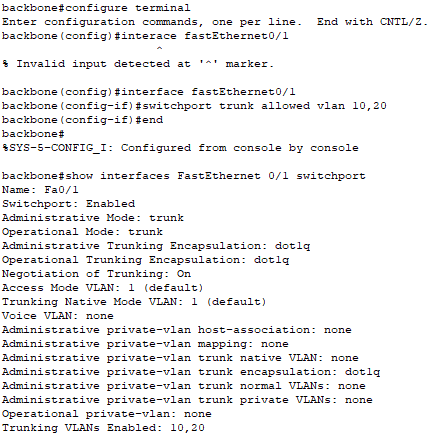
\includegraphics[width=\textwidth]{./img/Backbone/Access1.png}
        \subcaption{Verbindung zu Access1 einstellen}
    \end{subfigure}
\end{figure}
\begin{figure}[!htb]\ContinuedFloat
    \centering
    \begin{subfigure}{\textwidth}
        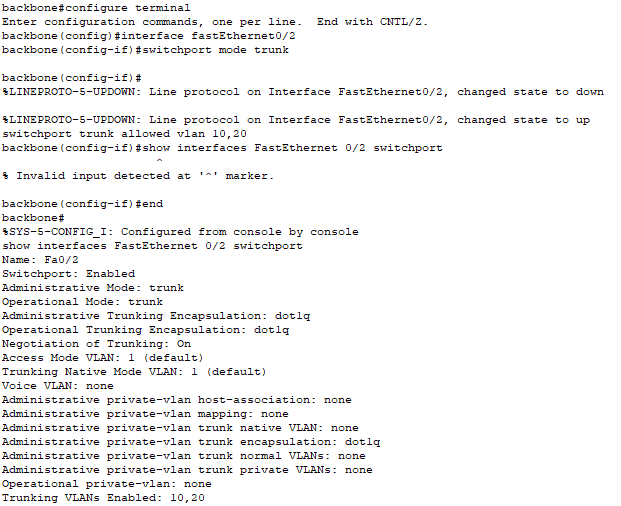
\includegraphics[width=\textwidth,height=.8\textheight]{./img/Backbone/Access2.png}
        \subcaption{Verbindung zu Access2 einstellen}
    \end{subfigure}
\end{figure}
\FloatBarrier
